\documentclass{llncs}
\usepackage{amsmath,amssymb,calc,ifthen}
\usepackage{float}
%\usepackage{cancel}
\usepackage[table,usenames,dvipsnames]{xcolor} % for coloured cells in tables
\usepackage{tikz}
% Allows us to click on links and references!
\usepackage{hyperref}
\usepackage{url}
\hypersetup{
colorlinks,
citecolor=black,
filecolor=black,
linkcolor=black,
urlcolor=black
}
% Nice package for plotting graphs
% See excellent guide:
% http://www.tug.org/TUGboat/tb31-1/tb97wright-pgfplots.pdf
\usetikzlibrary{plotmarks,shapes}
\usepackage{amsmath,graphicx}
\usepackage{epstopdf}
\usepackage{caption}
\usepackage{subcaption}
\usepackage{graphicx}
% highlight - useful for TODOs and similar
\usepackage{color}
\newcommand{\hilight}[1]{\colorbox{yellow}{#1}}
\newcommand\ci{\perp\!\!\!\perp} % perpendicular sign
\newcommand*\rfrac[2]{{}^{#1}\!/_{#2}} % diagonal fraction
\newcommand\SLASH{\char`\\}
\usepackage{listings}
% margin size
\usepackage{pdfpages}
\usepackage{enumitem} % for nested enumerate numbers 1 1.1 1.1.1
% \usepackage{breqn}
% \usepackage[linesnumbered]{algorithm2e}
% \usepackage{algorithmicx,algpseudocode}
% \usepackage{wrapfig} % for allowing text wrapped around the algorithm
% \newcommand\mycommfont[1]{\footnotesize\ttfamily\textcolor{blue}{#1}}
% \SetCommentSty{mycommfont}

% \usepackage{titlesec}
% \titlespacing*{\section}
% {0pt}{5.5ex plus 1ex minus .2ex}{4.3ex plus .2ex}


\DeclareMathOperator*{\argmin}{arg\,min}
\DeclareMathOperator*{\argmax}{arg\,max}

\begin{document}

\definecolor{blue3}{HTML}{86B7FC} % med blue
\definecolor{blue1}{HTML}{B5F1FF} % light blue
\definecolor{blue2}{HTML}{E0F9FF} % very light blue

\title{Disease Knowledge Transfer for Alzheimer's Variants}
%
\titlerunning{Disease Knowledge Transfer across Alzheimer's Variants}  % abbreviated title (for running head)
%                                     also used for the TOC unless
%                                     \toctitle is used
%

% * <mrazvan22@gmail.com> 2018-03-02T16:41:47.321Z:
% 
% Author list: Me, Pere (helped with validation), Marco (used his code), Alex (writing+tadpole), Neil (tadpole),  Arman, Keir (DTI data), Seb, Danny
% 
% ^ <mrazvan22@gmail.com> 2018-03-02T16:55:06.003Z.


\maketitle              % typeset the title of the contribution

\begin{abstract}

We present Disease Knowledge Transfer (DKT), a technique for transferring biomarker correlations between Alzheimer's disease (AD) variants. DKT allows, for the first time, to infer biomarker values and their progressions in rare variants of AD for which data on such biomarkers is not available, by learning them from a different disease. For doing this, we formulate a new dementias paradigm called "Affected Overlap", which proposes that dementias are diseases that affect overlapping brain regions, and thus present certain biomarker characteristics that are shared and can thus be transferred across diseases. We then formulate the DKT model implementing this paradigm as a joint-disease generative model of biomarker progression which disentangles the biomarker correlations that are disease-specific from those correlations that are disease-agnostic. We demonstrate DKT on three datasets: (1) the TADPOLE Challenge dataset containing typical AD subjects (tAD) from the Alzheimer's Disease Neuroimaging Initiative (ADNI) dataset who had MRI, FDG-PET, AV45, AV1451 or DTI scans, as well as two datasets from our local centre containing subjects with (2) typical AD and (3) Posterior Cortical Atrophy (PCA) that have only undergone MRI scans. We train the DKT model on all three datasets at once, and show that it is able to predict, in PCA subjects, plausible population-level biomarker for FDG, DTI, AV45 and AV1451 biomarkers, for which no data was available. We validate the predictions of DKT using a small set of DTI scans for the PCA cohort. We demonstrate that DKT may be a useful tool to analyse and understand rare forms of dementias for which multimodal data is not available or is limited (e.g. cross-sectional). Finally, by leveraging data from multiple diseases, DKT also has the potential to provide more accurate disease staging compared to traditional disease progression models, which is useful for patient stratification in clinical trials.
% * <alexandra.young@ucl.ac.uk> 2018-03-02T17:28:57.289Z:
% 
% > Finally,
% You've got finally twice
% 
% ^ <alexandra.young@ucl.ac.uk> 2018-03-02T17:29:38.345Z:
% 
% Could put we demonstrate (or something a bit weaker)
%
% ^ <alexandra.young@ucl.ac.uk> 2018-03-02T19:02:52.149Z.


\keywords{Disease Progression Model, Transfer Learning, Manifold Learning, Alzheimer's Disease, Posterior Cortical Atrophy}
\end{abstract}

\section{Introduction}


% biomarkers in alzheimer's -> measuring the evolution helps staging in clinical trials
There currently exist several image-based biomarkers for Alzheimer's disease that can be used to track its progression: AV45 Positron Emission Tomography (PET) measuring amyloid-plaque aggregation, AV1451 PET measuring tau tangle aggregation, Flourodeoxyglucose (FDG) PET measuring brain hypometabolism, Magnetic Resonance Imaging (MRI) measuring structural integrity and Diffusion Tensor Imaging (DTI) measuring connectivity integrity. Measuring the exact evolution of these biomarkers over the disease progression can lead to better disease staging of patients, which helps stratification in clinical trials.


% hypothetical model has specific ordering of modality biomarkers -> ordering or spatial biomarkers (different dimension) -> spatial differences in different dementias -> network vulnerability hypothesis.
A hypothetical model of disease progression has been previously published by \cite{jack2010hypothetical}, which proposes that the first biomarkers to become abnormal are measures of amyloid beta aggregation, followed by tau abnormalities, hypometabolism, structural MRI-based measures and finally cognitive decline. While this hypothetical model proposes a modality-specific ordering of biomarkers in typical AD, it has also been observed that within the same modality, biomarker measurements have a spatial sequence of abnormality that correlates with Braak stages: hippocampal volumes and entorhinal measures become abnormal first, followed by other structures within the temporal lobe, followed by parietal and frontal abnormalities. However, the spatial ordering of abnormality differs in other Alzheimer's variants. For example, in Posterior Cortical Atrophy, posterior regions such as the occipital lobe and superior parietal regions have been shown to become affected. The network vulnerability theory by Seeley et al. \cite{seeley2009neurodegenerative} suggests that damage to specific underlying connectivity networks leads to spatially distinct patterns of neurodegeneration. There is nevertheless a great degree of heterogeneity within these diseases, which led some to suggest that subjects with different Alzheimer's variants lie on a continuum of phenotypical variation \cite{crutch2012posterior}. 
% * <alexandra.young@ucl.ac.uk> 2018-03-02T19:01:16.243Z:
% 
% > The network vulnerability theory by Seeley et al. \cite{seeley2009neurodegenerative} suggests that damage to specific underlying connectivity networks leads to spatially distinct patterns of neurodegeneration. There is nevertheless a great degree of heterogeneity within these diseases, which led some to suggest that subjects with different Alzheimer's variants lie on a continuum of phenotypical variation \cite{crutch2012posterior}. 
% The relationship between these two statements is unclear from the way its written
% 
% ^.

The amount of heterogeneity within each variant and the network vulnerability hypothesis by \cite{seeley2009neurodegenerative} suggest that it should be theoretically possible to perform transfer learning across Alzheimer's variants. While recent studies \cite{hon2017towards} tried to perform transfer learning by transferring knowledge from generic image datasets to Alzheimer's disease, we are not aware of any studies that have tried to transfer knowledge across different types of Alzheimer's variants or other dementias. Moreover, current transfer learning approaches focused only on improving diagnostic classification using supervised approaches. We are not aware of any study to date that has tried to estimate, through transfer learning, a continuous disease progression manifold that doesn't rely on diagnoses. There are two key benefits to performing transfer learning across dementia variants: 1. biomarker evolutions can be estimated in rare dementias for which there is not enough data (uni-modal datasets, few subjects, cross-sectional data only) and 2. adding extra information from other datasets can help with staging and biomarker trajectory estimation.

We propose Disease Knowledge Transfer, a generative model that estimates progression of multiple dementias simultaneously and which inherently performs transfer learning from one type of dementia to another. The model achieves this by disentangling \emph{disease-specific} biomarker correlations from \emph{disease-agnostic} correlations.  We fit the model simultaneously to three datasets: 1. the TADPOLE Challenge dataset containing subjects from the ADNI study containing MRI, FDG-PET, DTI, AV45 and AV1451 scans 2. MRI scans from typical AD subjects in our local centre and 3. MRI scans from patients with Posterior Cortical Atrophy (PCA) from our local centre. We then used the fitted model to predict non-MRI trajectories for PCA patients, which have been learned from the ADNI dataset. We finally validated the DTI trajectories in PCA using a small test set of 20 DTI scans from the PCA patients and controls from our local centre.
% * <alexandra.young@ucl.ac.uk> 2018-03-02T17:54:07.562Z:
% 
% > unsupervised
% Is it unsupervised or does it know which disease/dataset is which, in which case it's semi-supervised?
% 
% ^ <mrazvan22@gmail.com> 2018-03-02T18:05:17.625Z:
% 
% Model is indeed supervised with respect to dataset/disease, but unsupervised with respect to diagnosis within same disease (e.g. Control, MCI and AD in ADNI). I removed the supervised-ness though in order not to create confusion. 
%
% ^.


\begin{figure}[h]
 \centering
 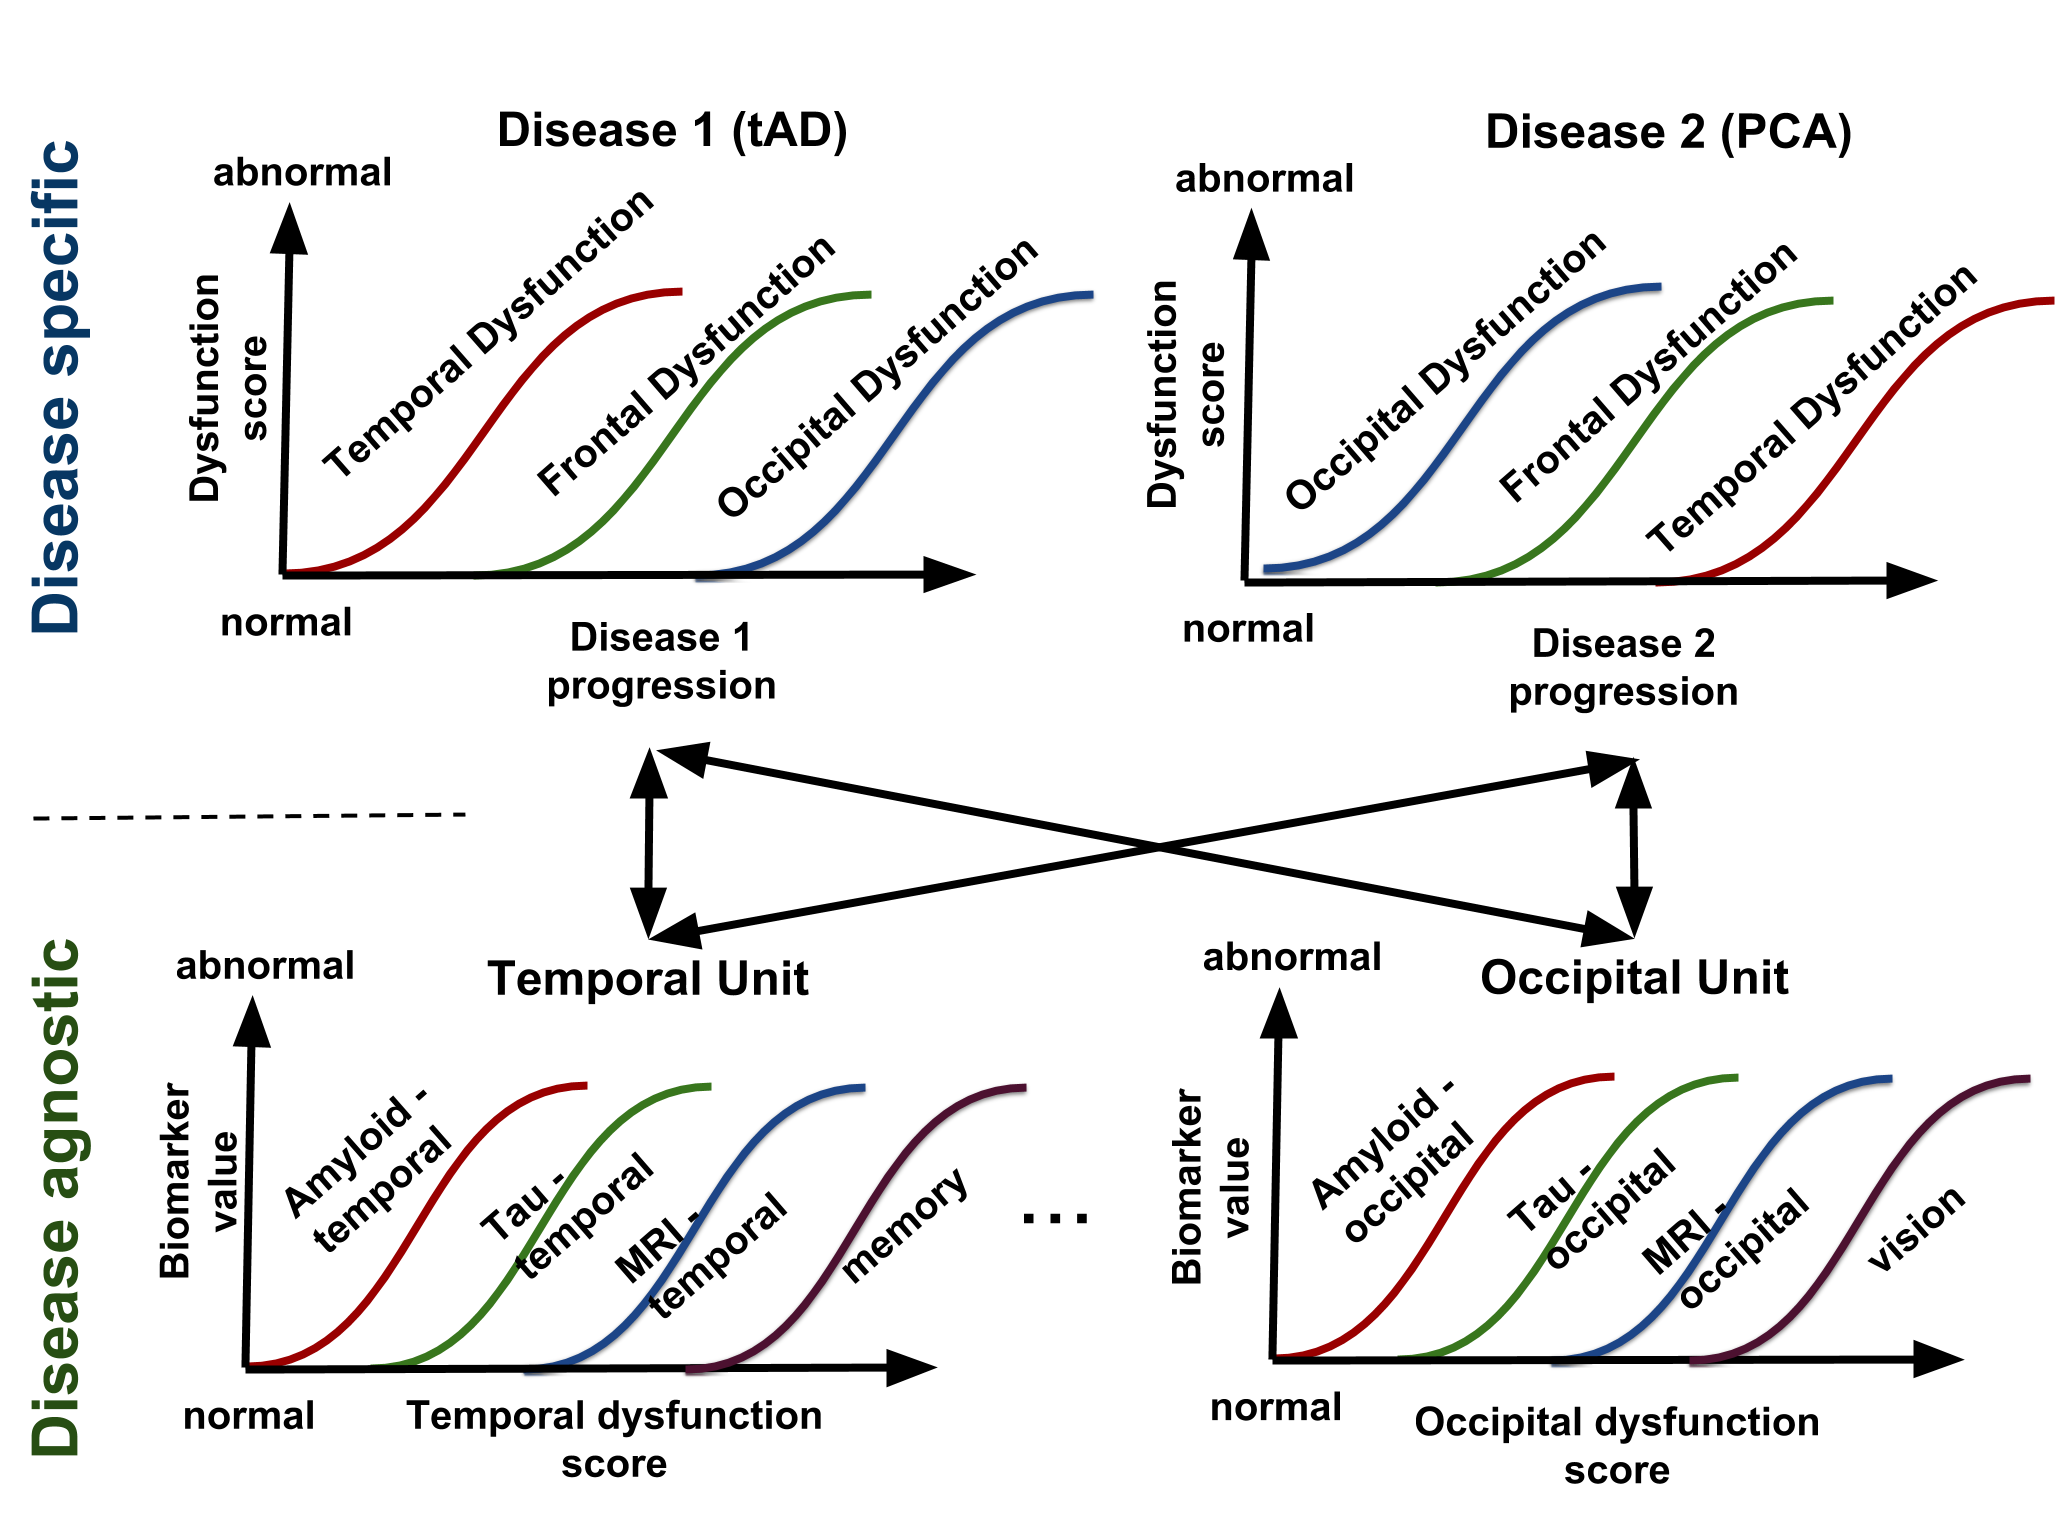
\includegraphics[width=\textwidth]{figures/disease_knowledge_transfer.png}
 \caption{Outline of the proposed framework for joint modelling of multiple diseases. We assume that each disease can be modelled as the evolution of some abstract dysfunctionality scores, each related to a brain region. Each dysfunctionality score is then assumed to be modelled as the progression of several biomarkers within that same region, but having different modalities. One key assumption of the model is that the biomarkers within each unit (bottom row) are disease agnostic (i.e. have the same dynamics for every disease), while the dysfunction scores (top row) are disease specific.}
\end{figure}

\subsection{Methods}

For modelling disease-agnostic correlations, we assume biomarkers are grouped into \emph{functional units}, where correlations within each unit are disease-agnostic (e.g. biomarkers corresponding to the same ROI).  Each biomarker is assigned a-priori to a specific functional unit, which corresponds to a brain region, say temporal lobe (Fig 1., bottom).  For example, biomarkers assigned to the temporal unit could be: amyloid in temporal lobe, tau in temporal lobe, MRI atrophy in temporal lobe and certain memory tests. Using a disease progression model of our choice, for each region-specific functional unit we can model the correlation of biomarkers within that functional unit (Figure 1, bottom), which allows us to reconstruct a region- or unit-specific \emph{dysfunction} progression axis which can be used for staging subjects. Finally, we express the disease specific correlations (Figure 1, top) not directly with each biomarkers, but via the dysfunction scores estimated within each functional unit.  

The proposed model is parsimonious, easily interpretable by abstracting away biomarker information into the functional units, and can be used for \emph{disease knowledge transfer}, i.e. learning correlations in one disease from another. Our approach is inspired by transfer learning methods from machine learning, but the model is generative, easing interpretability.


Variable names:
\begin{itemize}
 \item $\Lambda$ = set of \emph{functional units}, i.e. \{temporal, parietal, occipital, ..\}. Biomarkers belonging to the same functional unit are asusmed to have disease-agnostic correlations.
 \item $y_{ijk}$ = measurement in subject $i$, visit $j$, biomarker $k$
%  \item $d_{ijl}$ = dysfunctionality score in subject $i$, visit $j$ in \emph{functional unit} $l$, where $l \in \Lambda$
%  \item $s_{ij}$ = disease progression score in subject $i$, visit $j$
 \item $\theta_k$ = parameters of trajectory for biomarker $k$
 \item $\lambda^l$ = parameters of trajectory for functional unit $l$, where $l \in \Lambda$
 \item $\psi$ : \{1, ..., K\} $ \rightarrow Lambda$ is a function that maps beach biomarker to its corresponding functional unit
 \item $\beta_i$: time shift parameter for subject $i$ (disease specific)
 \item $\beta_i^{l}$: time shift parameter for subject $i$ used in functional unit $l$, where $l \in \Lambda$
 \item $\Omega$: set ${(i,j,k)}$ of measurements available from every subject $i$, visit $j$ in biomarker $k$
\end{itemize}

Likelihood for one single measurement in one subject visit: 
\begin{equation}
 p(y_{ijk}|\theta_k, \lambda^{\psi(k)}, \beta_i) = \sum_{\beta_i^{\psi(k)}} p(y_{ijk}| \beta_i^{\psi(k)}, \theta_k) p(\beta_i^{\psi(k)}| \lambda^{\psi(k)}, \beta_i)
\end{equation}

where $\beta_i^{\psi(k)}$ is a latent variable denoting the stage of subject $i$ in functional unit $\psi(k)$, where biomarker $k$ was assigned.

Extending the above to multiple, subjects, visits and biomarkers, we get the final model likelihood:
\begin{equation}
 p(y_{.,.,.}|\theta_1, ..., \theta_K, \{\lambda^{\psi(l)} | l \in \Lambda \}, \beta_1, ..., \beta_N) = \\ \prod_{(i,j,k) \in \Omega} \sum_{\beta_i^{\psi(k)}} p(y_{ijk}| \beta_i^{\psi(k)}, \theta_k) p(\beta_i^{\psi(k)}| \lambda^{\psi(k)}, \beta_i)
\end{equation}

Modelling of $p(y_{ijk}| \beta_i^{\psi(k)}, \theta_k)$ and $p(\beta_i^{\psi(k)}| \lambda^{\psi(k)}, \beta_i)$ will be done with a non-parametric model (Gaussian Process, Lorenzi et al., 2017)


Let's assume we have MRI and PET data in tAD (from ADNI), but only MRI data for another disease, e.g. PCA. We can model the disease-agnostic region-specific relationship between MRI and PET, and also build the disease specific progression models for tAD (using MRI and PET) and PCA (using MRI only). Finally, our model allows us to propagate the knowledge of PET dynamics in tAD to PCA subjects, without using any PET scans from PCA patients. This can be done by maximising the following likelihood (assuming we already have a model for tAD):

\begin{equation}
 p(y_{.,.,.}^{PCA}|\theta_1^{tAD}, ..., \theta_K^{tAD}, \{\lambda^{\psi(l)^{PCA}} | l \in \Lambda \}, \beta_1^{PCA}, ..., \beta_N^{PCA}) = 
\end{equation}

 \begin{equation}
 \prod_{(i,j,k) \in \Omega} \sum_{\beta_i^{\psi(k)}} p(y_{ijk}^{PCA}| \beta_i^{\psi(k)}, \theta_k^{tAD}) p(\beta_i^{\psi(k)}| \lambda^{\psi(k)^{PCA}}, \beta_i^{PCA})
\end{equation}

\section{Results}

Fig. \ref{fig:occipUnit} shows the estimated biomarker trajectories within the \emph{occipital unit}, along with samples from the model posterior and aligned subject data. The model shows a good data fit, and we can observe most PCA subjects having abnormal occipital volumes, thus leading to high occipital dysfunctionality scores, in line with the current understanding of PCA as affecting posterior regions \cite{crutch2012posterior}. Fig. \ref{fig:occipUnit} shows the progression of dysfunctionality scores for (a) typical AD and (b) PCA. In typical AD, we see that temporal dysfunction becomes abnormal  

\newcommand{\expFld}{figures}

% data fitting within one unit
\begin{figure}[H]
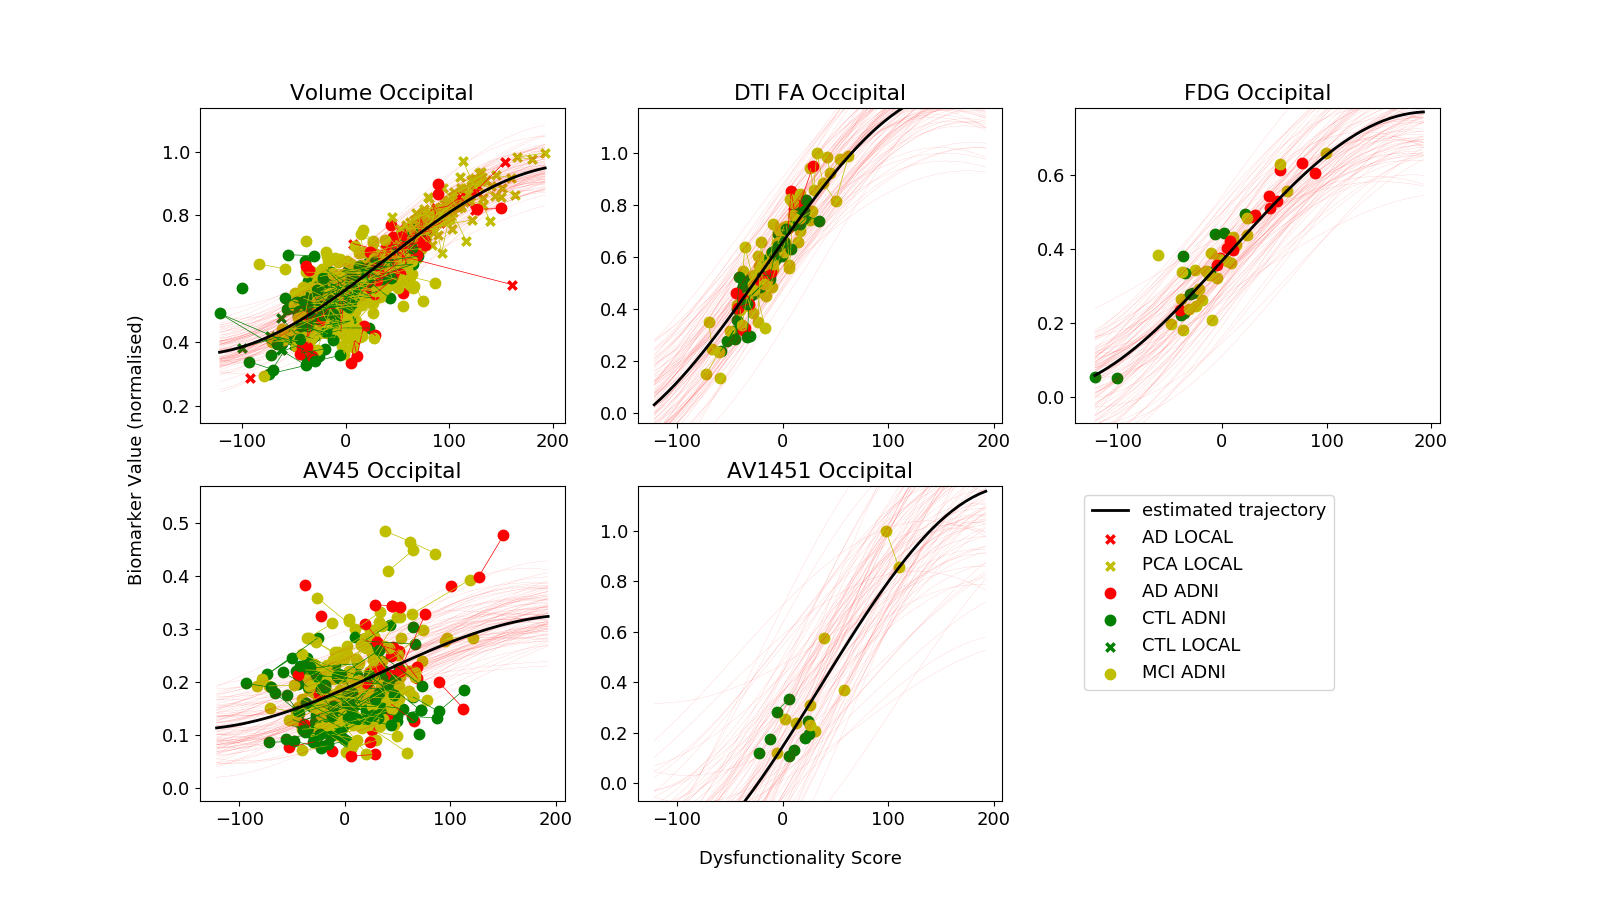
\includegraphics[width=\textwidth, trim=90 0 110 0, clip]{figures/unit1_allTraj_tad-drcTinyPen1_JMD.png} 
\caption{Estimated biomarker trajectories in the Occipital Unit. Subject data from ADNI and our local cohort are also shown. The X-axis represents, defined as the occipital dysfunctionality score, represents the time-shifts (in months) of each subject. Red lines represent samples from the trajectory posterior. The Y-axis represents biomarker values which have been normalised to the [0,1] range.}
\label{fig:occipUnit}
\end{figure}




% PCA vs tAD disease space
\begin{figure}[H]
\begin{subfigure}{0.47\textwidth}
\centering
typical AD\\
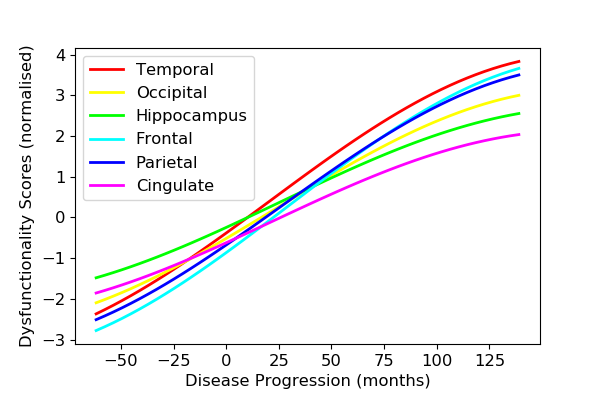
\includegraphics[width=\textwidth, trim=0 0 0 20, clip]{figures/tAD_trajSameSpace_tad-drcTinyPen1_JMD.png} 
\caption{}
\end{subfigure}
\begin{subfigure}{0.47\textwidth}
\centering
PCA\\
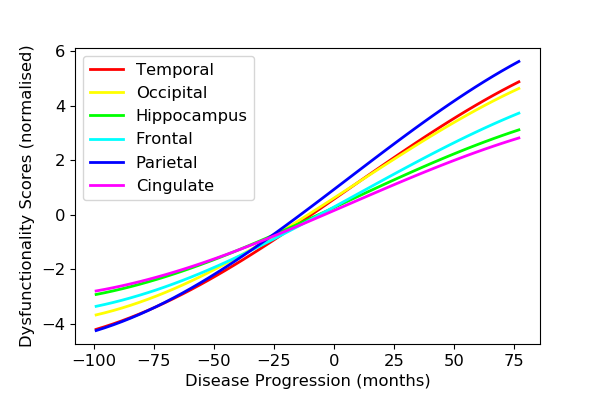
\includegraphics[width=\textwidth, trim=0 0 0 20, clip]{figures/PCA_trajSameSpace_tad-drcTinyPen1_JMD.png} 
\caption{}
\end{subfigure}
\caption{Progression of dysfunctionality scores for (a) typical AD and (b) PCA. In typical AD, we notice that the temporal scores are most affected after the disease }
\label{fig:pcaTadDisSpace}
\end{figure}

% estimated (hypothetical) trajectories in PCA: DTI, FDG, AV45, AV1451.Volumetric trajectories were based on PCA MRI data.
\begin{figure}[H]
 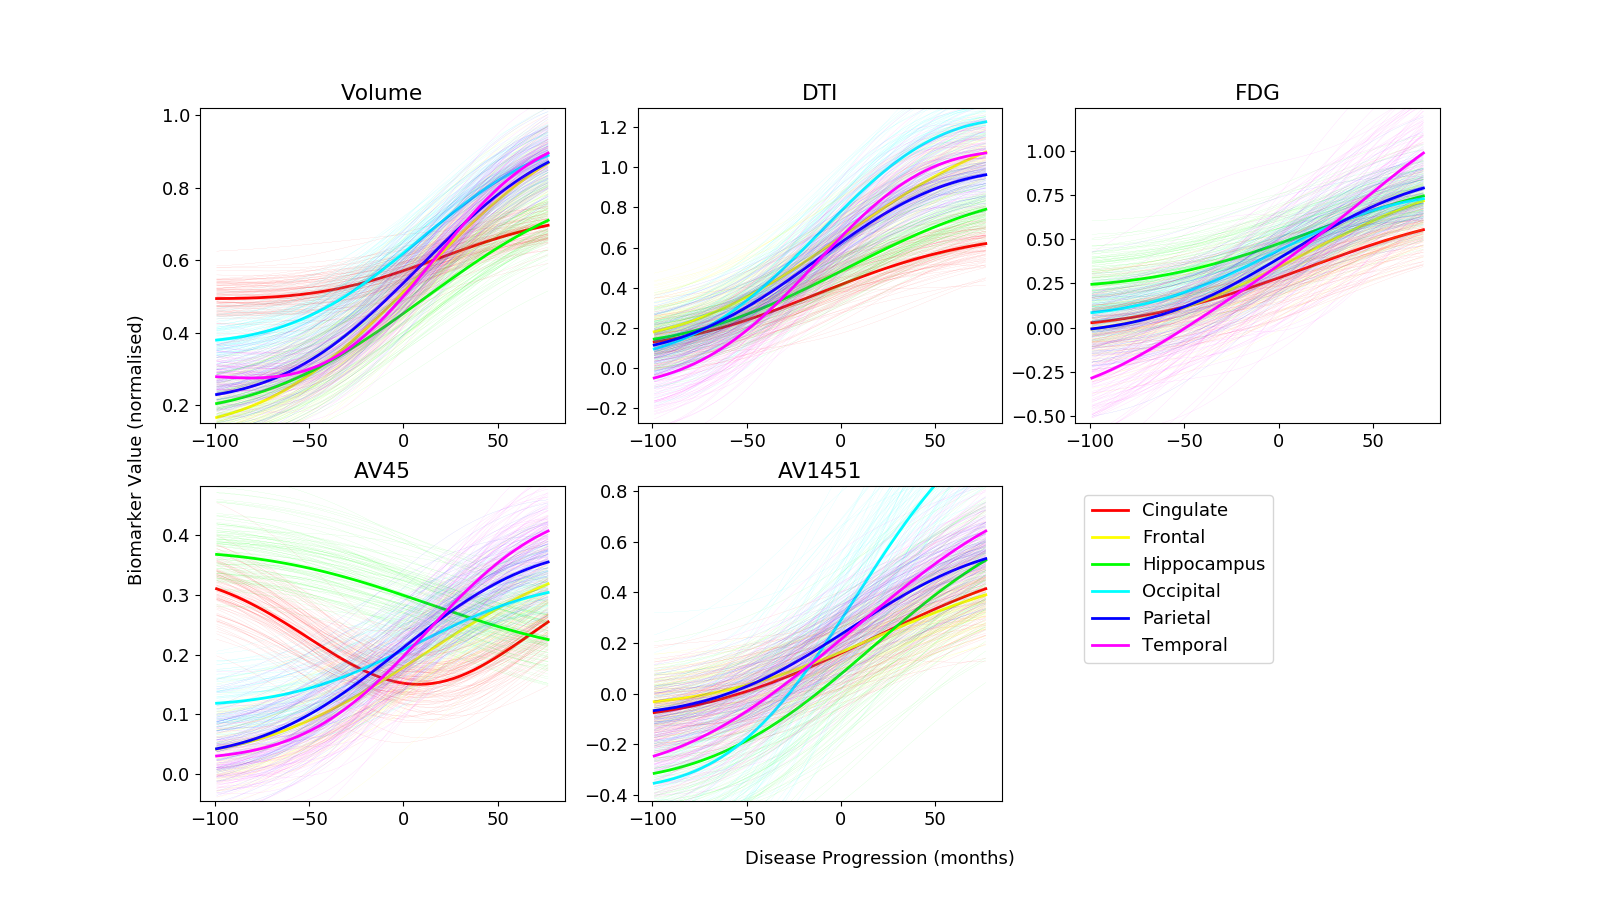
\includegraphics[width=\textwidth, trim=0 0 0 0, clip]{figures/trajDisSpaceOverlap_PCA_tad-drcTinyPen1_JMD.png}
 \caption{Estimated trajectories for the PCA cohort. The only data that was available was the MRI volumetric data. The dynamics of the other biomarkers has been inferred by the model using data from typical AD, and taking into account the different spatial distribution of pathology in PCA as compared to typical AD.}
 \label{fig:PCAtrajByModality}
\end{figure}
% * <mrazvan22@gmail.com> 2018-03-02T15:58:16.565Z:
% 
% some trajectories in AV45 screwed up due to bad initial starting point. Will try to re-fit the model if I have time.
% 
% ^.


\section*{Validation}

% LOCAL DTI validation

\begin{figure}[H]
 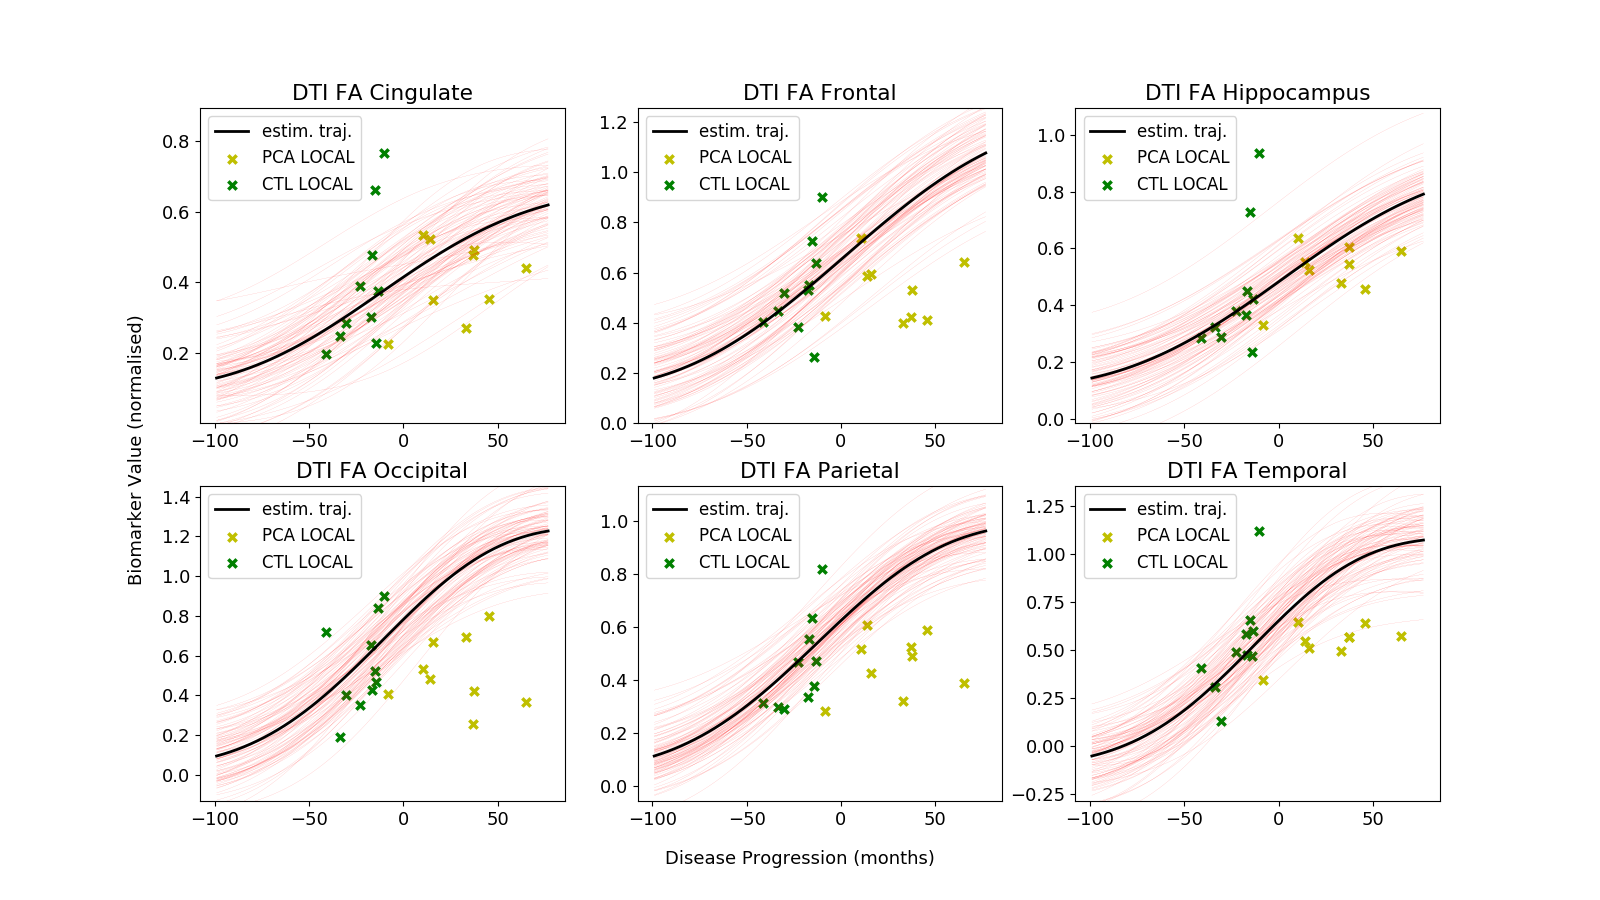
\includegraphics[width=\textwidth, trim=0 0 0 0, clip]{figures/validDtiPCA.png}
 \caption{Validation of the Disease Knowledge Transfer Model using DTI data of PCA subjects from our local cohort. No DTI data, or other non-MRI data from PCA subjects was used to fit the model. The estimated trajectories seem to approximate the data reasonably well in temporal, hippocampus and cingulate regions, and less well in the other regions.}
\label{fig:DTIvalid}
\end{figure}

\section{Acknowledgements}

This work was supported by the EPSRC Centre For Doctoral Training in Medical Imaging with grant EP/L016478/1. AE received a McDonald Fellowship from the Multiple Sclerosis International Federation (MSIF, www.msif.org), and the ECTRIMS - MAGNIMS Fellowship. ALY was supported through an EPSRC Doctoral Prize Fellowship. NPO and SG received funding from the EU Horizon 2020 research and innovation programme under grant agreement No 666992. SJC was supported by an Alzheimer’s Research UK Senior Research Fellowship and ESRC/NIHR (ES/L001810/1) and EPSRC (EP/M006093/1) grants. DCA's work on this topic has funding from the EU Horizon 2020 research and innovation programme under grant agreement No 666992, as well as EPSRC grants J020990, M006093 and M020533. Data collection and sharing for this project was funded by the Alzheimer's Disease Neuroimaging Initiative (ADNI) (National Institutes of Health Grant U01 AG024904) and DOD ADNI (Department of Defense award number W81XWH-12-2-0012). The Dementia Research Centre is an ARUK coordination center.


%
% ---- Bibliography ---- 
% USE HARVARD STANDARD

\bibliographystyle{unsrtnat}
\begin{thebibliography}{5}

\bibitem{jack2010hypothetical}
Jack, C.R., Knopman, D.S., Jagust, W.J., Shaw, L.M., Aisen, P.S., Weiner, M.W., Petersen, R.C. and Trojanowski, J.Q., 2010. Hypothetical model of dynamic biomarkers of the Alzheimer's pathological cascade. The Lancet Neurology, 9(1), pp.119-128.

\bibitem{fonteijn2012event}
Fonteijn, H.M., Modat, M., Clarkson, M.J., Barnes, J., Lehmann, M., Hobbs, N.Z., Scahill, R.I., Tabrizi, S.J., Ourselin, S., Fox, N.C. and Alexander, D.C., 2012. An event-based model for disease progression and its application in familial Alzheimer's disease and Huntington's disease. NeuroImage, 60(3), pp.1880-1889.

\bibitem {jedynak2012}
Jedynak, B.M., Lang, A., Liu, B., Katz, E., Zhang, Y., Wyman, B.T., Raunig, D., Jedynak, C.P., Caffo, B., Prince, J.L. and Alzheimer's Disease Neuroimaging Initiative, 2012. A computational neurodegenerative disease progression score: method and results with the Alzheimer's Disease Neuroimaging Initiative cohort. Neuroimage, 63(3), pp.1478-1486.

\bibitem{donohue2014estimating}
Donohue, M.C., Jacqmin-Gadda, H., Le Goff, M., Thomas, R.G., Raman, R., Gamst, A.C., Beckett, L.A., Jack, C.R., Weiner, M.W., Dartigues, J.F. and Aisen, P.S., 2014. Estimating long-term multivariate progression from short-term data. Alzheimer's \& Dementia, 10(5), pp.S400-S410.

\bibitem{schiratti2015mixed}
Schiratti, J.B., Allassonniere, S., Routier, A., Colliot, O., Durrleman, S. and Alzheimers Disease Neuroimaging Initiative, 2015, June. A mixed-effects model with time reparametrization for longitudinal univariate manifold-valued data. In International Conference on Information Processing in Medical Imaging (pp. 564-575). Springer International Publishing.


\bibitem{seeley2009neurodegenerative}
Seeley, W.W., Crawford, R.K., Zhou, J., Miller, B.L. and Greicius, M.D., 2009. Neurodegenerative diseases target large-scale human brain networks. Neuron, 62(1), pp.42-52.

\bibitem{crutch2012posterior}
Crutch, S.J., Lehmann, M., Schott, J.M., Rabinovici, G.D., Rossor, M.N. and Fox, N.C., 2012. Posterior cortical atrophy. The Lancet Neurology, 11(2), pp.170-178.

\bibitem{hon2017towards}
Hon, M. and Khan, N., 2017. Towards Alzheimer's Disease Classification through Transfer Learning. arXiv preprint arXiv:1711.11117.

\end{thebibliography}

\clearpage

\end{document}

